\documentclass[aspectratio=169]{beamer}
\usetheme[style=noir]{fhtw}
\usepackage{preamble}
\resetcounteronoverlays{listing}

\title[TensorFlow Lite]{TensorFlow Lite}
\subtitle{\glsentrytext{ci} - ASSIST \glsentrytext{heidi}}
\author{Alija Sabic, \glsentrytext{msc}}
\mail{sabic@technikum-wien.at}
\institute{Department Electronic Engineering}

\begin{document}

\begin{frame}[plain]
    \titlepage
\end{frame}

\section{Introduction}

\begin{frame}
    \begin{figure}
        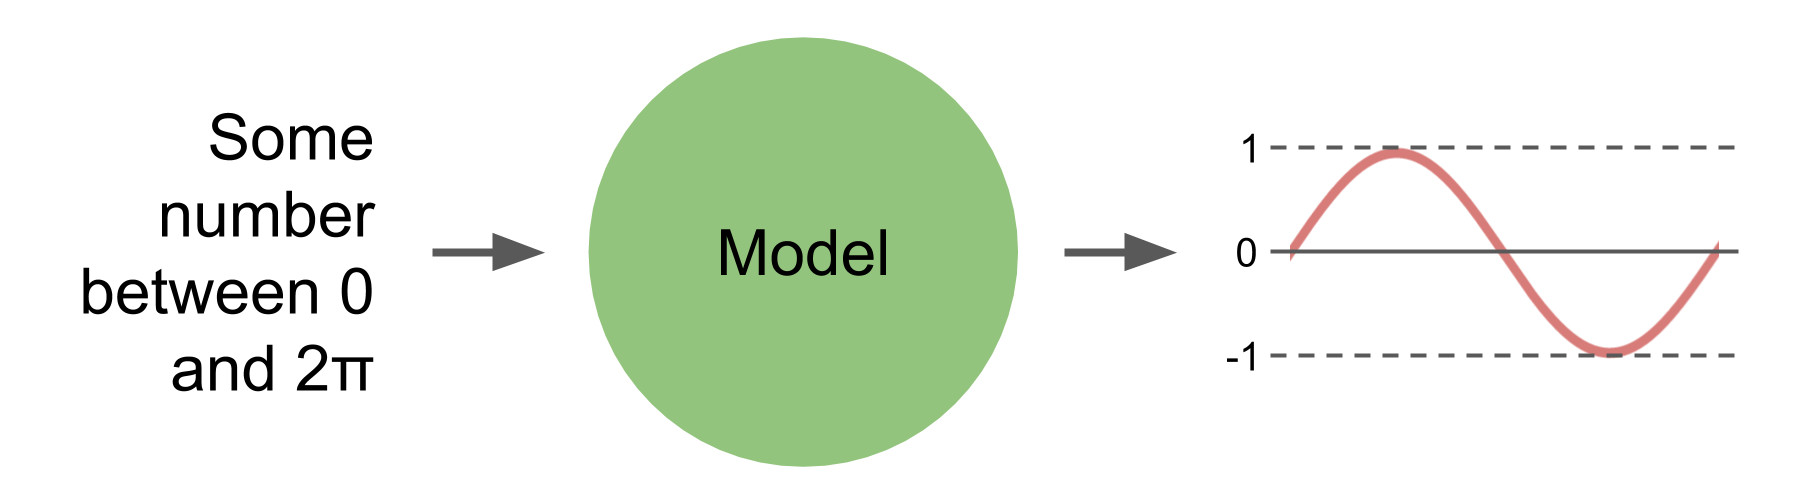
\includegraphics[width=0.85\textwidth]{images/tflite/sinewave-model-overview.jpg}
        \caption{Goal description.}
    \end{figure}
\end{frame}

\section{Model}
\subsection{Design}
\begin{frame}
    \begin{listing}[H]
        \inputsource[fontsize=\fontsize{10}{10}, firstline=66, lastline=76]{py}{tflite/tflite_sinewave_training.py}
        \caption{Create the model.}
        \label{lst:tflite:sinewave:model}
    \end{listing}
\end{frame}

\begin{frame}
    \begin{figure}
        \frame{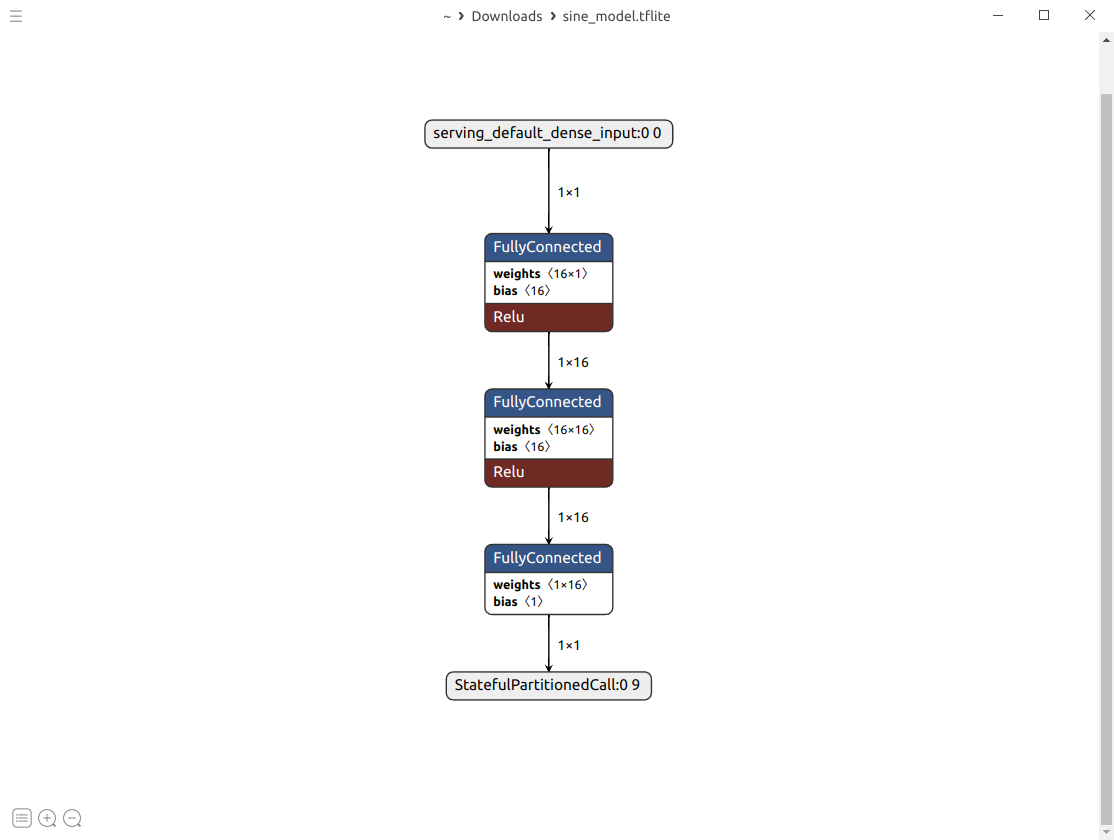
\includegraphics[width=0.85\textwidth]{images/tflite/netron.png}}
        \caption{Generated model with fully connected layers (\href{https://github.com/lutzroeder/netron}{Netron}).}
    \end{figure}
\end{frame}
\subsection{Google Colab}
\begin{frame}
    \par Open \href{https://colab.research.google.com/}{Google Colab} and create a new notebook.
    \begin{listing}[H]
        \inputsource[firstline=10, lastline=14]{py}{tflite/tflite_sinewave_training.py}
        \caption{IPython magic.}
        \label{lst:tflite:sinewave:magic}
    \end{listing}
\end{frame}
\subsection{Import}
\begin{frame}
    \begin{listing}[H]
        \inputsource[firstline=16, lastline=20]{py}{tflite/tflite_sinewave_training.py}
        \caption{Import dependencies.}
        \label{lst:tflite:sinewave:import}
    \end{listing}
    \begin{listing}[H]
        \inputsource[firstline=22, lastline=26]{py}{tflite/tflite_sinewave_training.py}
        \caption{Print version information.}
        \label{lst:tflite:sinewave:version}
    \end{listing}
\end{frame}
\subsection{Settings}
\begin{frame}
    \begin{listing}[H]
        \inputsource[firstline=13, lastline=20]{c}{arduino/sinewave-test.c}
        \caption{Project code: settings.}
        \label{lst:arduino:tflite:sinewave:settings}
    \end{listing}
\end{frame}
\subsection{Samples}
\begin{frame}
    \begin{listing}[H]
        \inputsource[fontsize=\fontsize{9}{9}, firstline=41, lastline=64]{py}{tflite/tflite_sinewave_training.py}
        \caption{Generate random samples.}
        \label{lst:tflite:sinewave:generate_samples}
    \end{listing}
\end{frame}

\begin{frame}
    \begin{figure}
        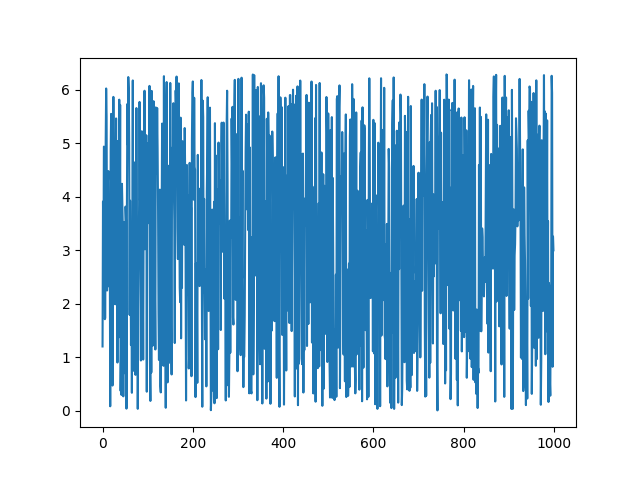
\includegraphics[width=0.85\textwidth]{images/tflite/colab/x-values.png}
        \caption{Random samples (x values).}
    \end{figure}
\end{frame}

\begin{frame}
    \begin{figure}
        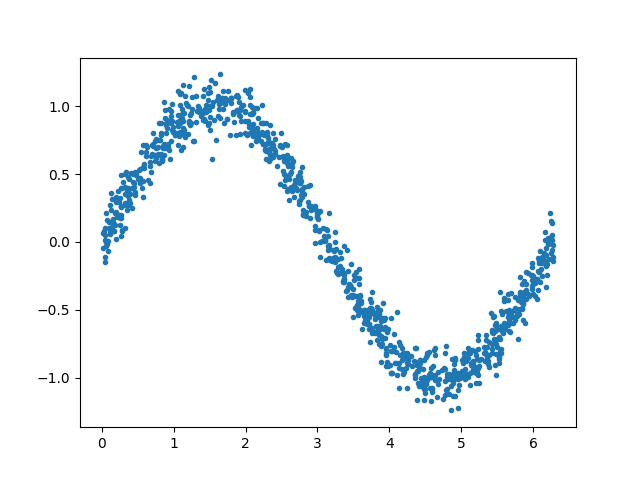
\includegraphics[width=0.85\textwidth]{images/tflite/colab/y-values.png}
        \caption{Random samples (y values).}
    \end{figure}
\end{frame}

\begin{frame}
    \begin{figure}
        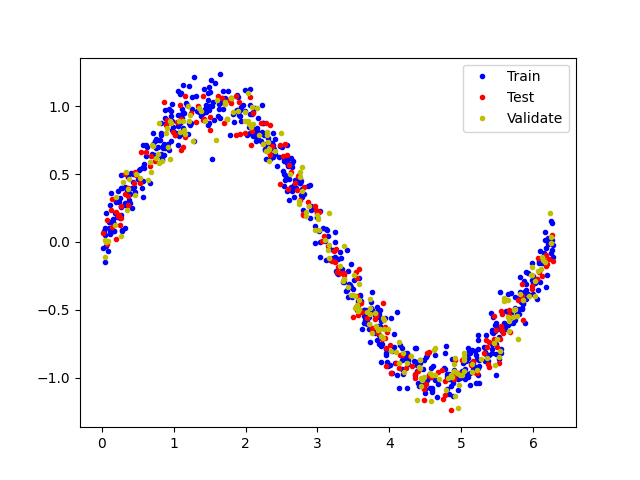
\includegraphics[width=0.85\textwidth]{images/tflite/colab/sets.png}
        \caption{Random sample sets: training, validation, test.}
    \end{figure}
\end{frame}
\subsection{Model}
\begin{frame}
    \begin{listing}[H]
        \inputsource[fontsize=\fontsize{10}{10}, firstline=66, lastline=76]{py}{tflite/tflite_sinewave_training.py}
        \caption{Create the model.}
        \label{lst:tflite:sinewave:model}
    \end{listing}
\end{frame}

\begin{frame}
    \begin{figure}
        \frame{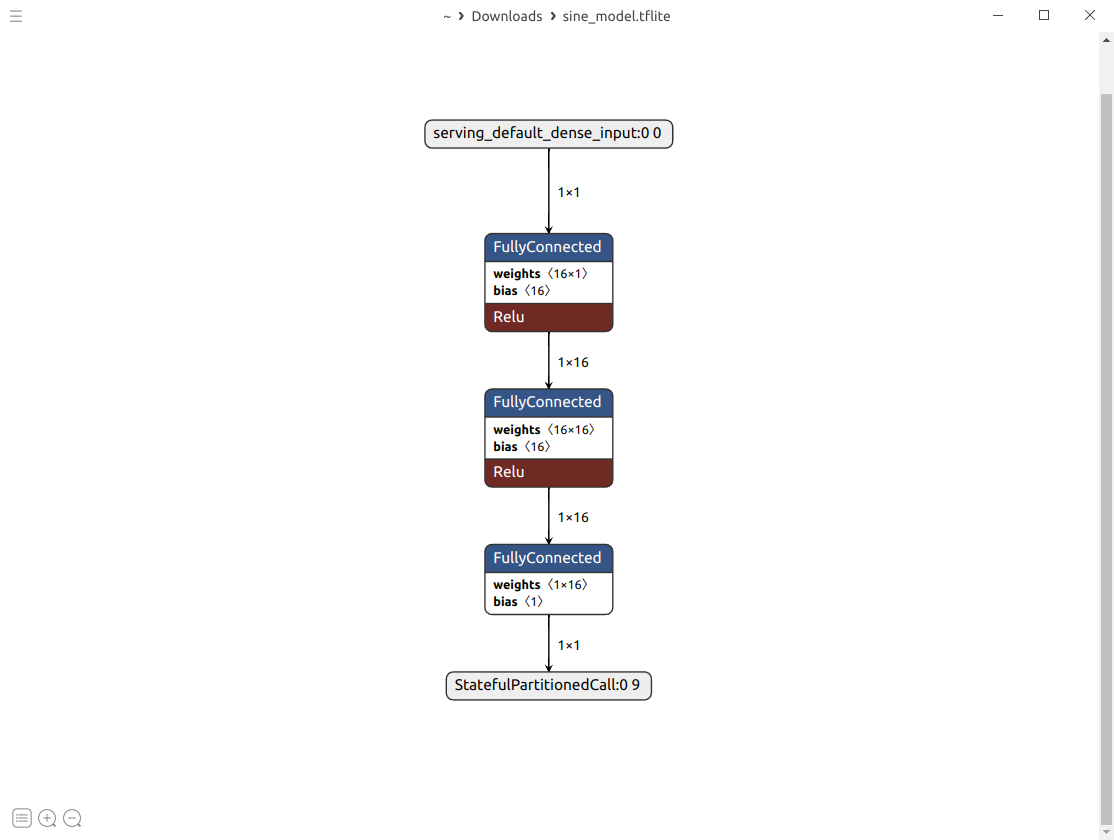
\includegraphics[width=0.85\textwidth]{images/tflite/netron.png}}
        \caption{Generated model with fully connected layers (\href{https://github.com/lutzroeder/netron}{Netron}).}
    \end{figure}
\end{frame}
\subsection{Train}
\begin{frame}
    \begin{listing}[H]
        \inputsource[fontsize=\fontsize{10}{10}, firstline=78, lastline=95]{py}{tflite/tflite_sinewave_training.py}
        \caption{Train the model.}
        \label{lst:tflite:sinewave:train}
    \end{listing}
\end{frame}

\begin{frame}
    \begin{figure}
        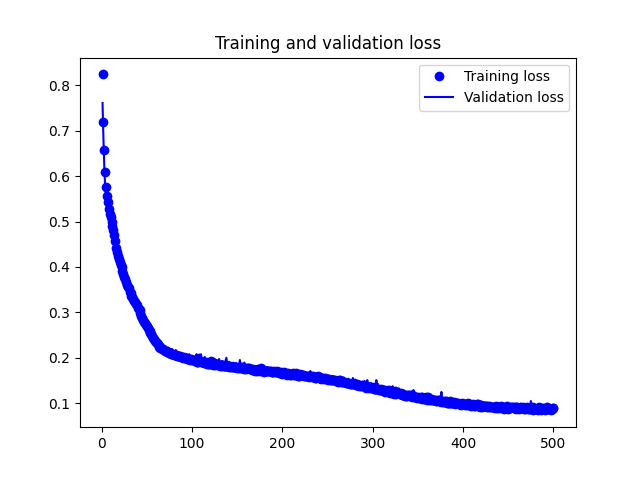
\includegraphics[width=0.85\textwidth]{images/tflite/colab/history.png}
        \caption{Training and validation loss.}
    \end{figure}
\end{frame}
\subsection{Test}
\begin{frame}
    \begin{listing}[H]
        \inputsource[firstline=97, lastline=105]{py}{tflite/tflite_sinewave_training.py}
        \caption{Test the model.}
        \label{lst:tflite:sinewave:test}
    \end{listing}
\end{frame}

\begin{frame}
    \begin{figure}
        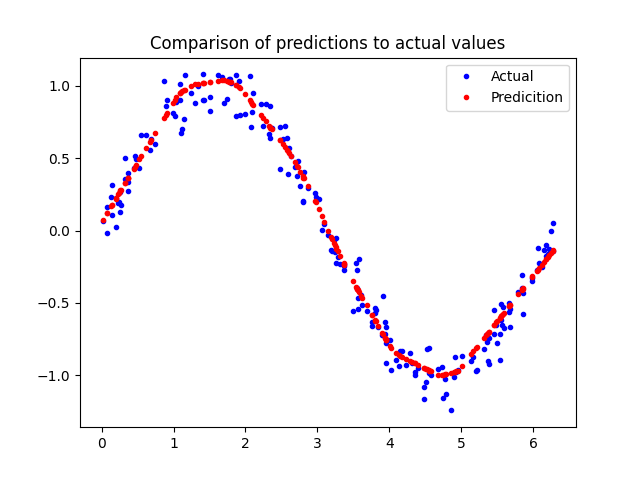
\includegraphics[width=0.85\textwidth]{images/tflite/colab/test.png}
        \caption{Model validation.}
    \end{figure}
\end{frame}
\subsection{Convert}
\begin{frame}
    \par The TensorFlow Lite Model file can be inspected with programs such as \href{https://github.com/lutzroeder/netron}{Netron} (\href{https://netron.app/}{Netron Browser App}).
    \begin{listing}[H]
        \inputsource[fontsize=\fontsize{9}{10}, firstline=107, lastline=112]{py}{tflite/tflite_sinewave_training.py}
        \caption{Convert to TensorFlow Lite model.}
        \label{lst:tflite:sinewave:tflite_model}
    \end{listing}
    \begin{listing}[H]
        \inputsource[fontsize=\fontsize{9}{10}, firstline=142]{py}{tflite/tflite_sinewave_training.py}
        \caption{Convert to C source file.}
        \label{lst:tflite:sinewave:tflite_model:c}
    \end{listing}
\end{frame}

\begin{frame}
    \begin{listing}[H]
        \inputsource[fontsize=\fontsize{9}{10}, firstline=114, lastline=140]{py}{tflite/tflite_sinewave_training.py}
        \caption{Converter function.}
        \label{lst:tflite:sinewave:tflite_model:c:converter}
    \end{listing}
\end{frame}

\section{Inference}
\subsection{Installation}
\begin{frame}[fragile]
    \par The officially supported TensorFlow Lite Micro library for Arduino\textregistered{} resides in the \href{https://github.com/tensorflow/tflite-micro-arduino-examples}{tflite-micro-arduino-examples} GitHub repository.
    \par To install the in-development version of this library, you can use the latest version directly from the GitHub repository.
    This requires you clone the repo into the folder that holds libraries for the Arduino\textregistered{} \acs{ide}.
    \par The location for this folder varies by operating system, but typically it's in \texttt{\textasciitilde{}/Arduino/libraries} (Linux), \texttt{\textasciitilde{}/Documents/Arduino/libraries/} (Mac\acs{os}), and \texttt{My Documents\textbackslash{}Arduino\textbackslash{}Libraries} (Windows).
    \begin{listing}[H]
        \begin{mdframed}
            \begin{minted}[autogobble, fontsize=\fontsize{7}{7}, linenos=false]{sh}
                git clone https://github.com/tensorflow/tflite-micro-arduino-examples Arduino_TensorFlowLite
            \end{minted}
        \end{mdframed}
        \caption{Download TensorFlow Lite.}
        \label{lst:tflite:installation}
    \end{listing}
\end{frame}
\subsection{Project}
\begin{frame}[fragile]
    \par Create a new project using the Arduino\textregistered{} \acs{ide} and copy the file (\texttt{sine\_model.h}, downloaded from Google) Colab to your project folder.
    \begin{listing}[H]
        \inputsource[fontsize=\fontsize{8}{8}, lastline=7]{c}{arduino/sine_model.h}[hidealllines=true, tikzsetting={draw=black, line width=0.35pt}, leftline=true, rightline=true, topline=true]
        \vspace{-1.25em}
        \begin{mdframed}[hidealllines=true, tikzsetting={draw=black, line width=0.35pt}, leftline=true, rightline=true]
            \begin{minted}[gobble=14, fontsize=\fontsize{8}{8}, linenos=false]{c}
                ...
            \end{minted}
        \end{mdframed}
        \vspace{-1.25em}
        \inputsource[fontsize=\fontsize{8}{8}, firstline=268]{c}{arduino/sine_model.h}[hidealllines=true, tikzsetting={draw=black, line width=0.35pt}, leftline=true, rightline=true, bottomline=true]
        \caption{Created model as C array (\texttt{sine\_model.h}).}
        \label{lst:tflite:sinewave:model:c_array}
    \end{listing}
    \par Alternatively, you can create a \texttt{C/C++} source file using \texttt{xxd} (Linux).
    \begin{listing}[H]
        \begin{mdframed}
            \begin{minted}[autogobble, linenos=false]{sh}
                xxd -i sine_model.tflite > sine_model.cc
            \end{minted}
        \end{mdframed}
        \caption{Download TensorFlow Lite.}
        \label{lst:tflite:sinewave:model:conversion}
    \end{listing}
\end{frame}
\subsection{Circuit}
\begin{frame}
    \begin{figure}
        \begin{tikzpicture}
            \ctikzset{bipoles/length=1cm, !vi/.style={no v symbols, no i symbols}, bipole voltage style/.style={text opacity=0}, bipole current style/.style={color=ttw-red}}
            \draw (2,4) node[rp2040] (rp20401) {}
            (rp20401.D2) to ++(1,0) to ++(0,4) to ++(2,0) to ++(0,-1) to [R,name=R,l={$R_1 = \SI{220}{\ohm}$},v=$U_1$,voltage shift=3.5,!vi] ++(0,-1) to [leDo,name=LED,l=$D_1$,v=$U_2$,i=$i$,voltage shift=3.5,!vi] ++(0,-2)
            (rp20401.GNDR) to ++(3,0) to ++(0,1);
            \fixedvlen[0.5cm]{R}{$U_1$}[tw-blue]
            \fixedvlen[0.5cm]{LED}{$U_2$}[tw-blue]
            \iarronly{LED}
        \end{tikzpicture}
        \caption{Project Circuit.}
    \end{figure}
\end{frame}
\subsection{Imports}
\begin{frame}
    \begin{listing}[H]
        \inputsource[fontsize=\fontsize{9}{9}, lastline=11]{c}{arduino/sinewave-test.c}
        \caption{Project code: import dependencies.}
        \label{lst:arduino:tflite:sinewave:import_define}
    \end{listing}
\end{frame}
\subsection{Settings}
\begin{frame}
    \begin{listing}[H]
        \inputsource[firstline=13, lastline=20]{c}{arduino/sinewave-test.c}
        \caption{Project code: settings.}
        \label{lst:arduino:tflite:sinewave:settings}
    \end{listing}
\end{frame}
\subsection{Globals}
\begin{frame}
    \begin{listing}[H]
        \inputsource[fontsize=\fontsize{9}{9}, firstline=22, lastline=35]{c}{arduino/sinewave-test.c}
        \caption{Project code: global variables.}
        \label{lst:arduino:tflite:sinewave:globals}
    \end{listing}
\end{frame}
\subsection{Setup}
\subsubsection{Logging}
\begin{frame}
    \begin{listing}[H]
        \inputsource[firstline=38, lastline=48]{c}{arduino/sinewave-test.c}
        \caption{Project code: error logging.}
        \label{lst:arduino:tflite:sinewave:setup:logging}
    \end{listing}
\end{frame}
\subsubsection{Model}
\begin{frame}
    \begin{listing}[H]
        \inputsource[fontsize=\fontsize{10}{10}, firstline=66, lastline=76]{py}{tflite/tflite_sinewave_training.py}
        \caption{Create the model.}
        \label{lst:tflite:sinewave:model}
    \end{listing}
\end{frame}

\begin{frame}
    \begin{figure}
        \frame{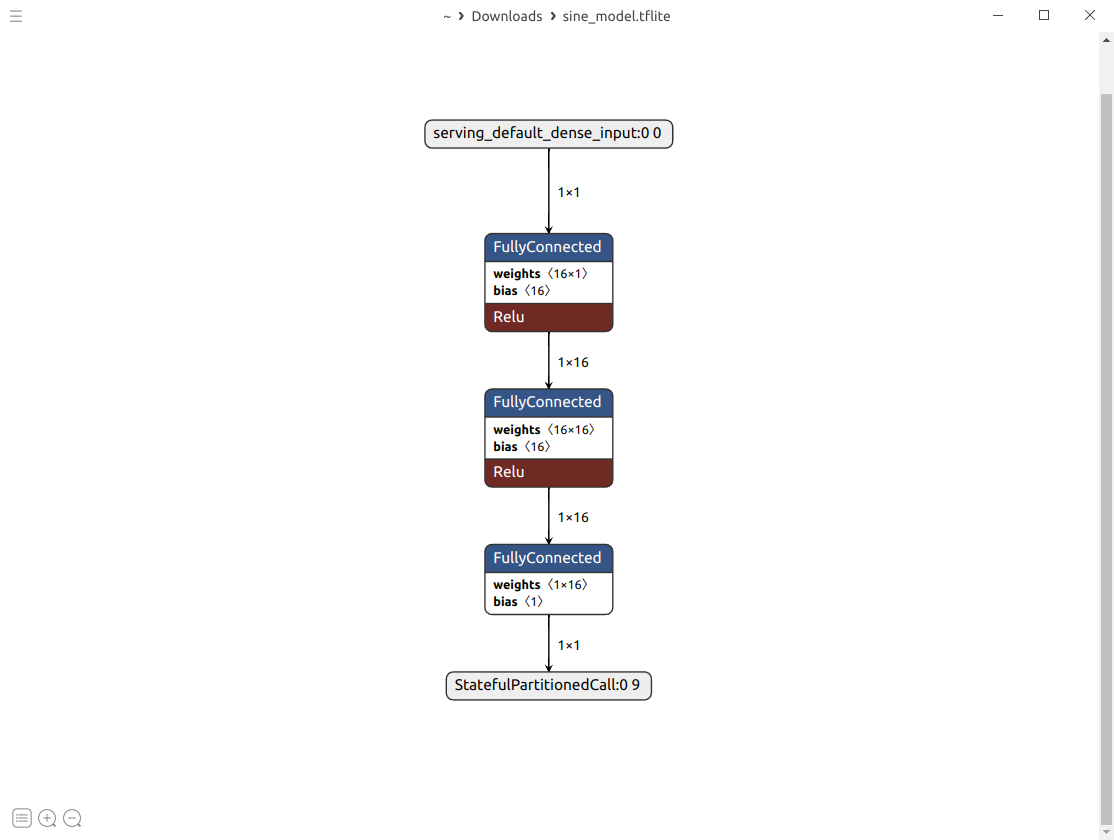
\includegraphics[width=0.85\textwidth]{images/tflite/netron.png}}
        \caption{Generated model with fully connected layers (\href{https://github.com/lutzroeder/netron}{Netron}).}
    \end{figure}
\end{frame}
\subsubsection{Interpreter}
\begin{frame}
    \begin{listing}[H]
        \inputsource[fontsize=\fontsize{9}{10}, firstline=65, lastline=80]{c}{arduino/sinewave-test.c}
        \caption{Project code: create an interpreter.}
        \label{lst:arduino:tflite:sinewave:setup:interpreter}
    \end{listing}
\end{frame}
\subsubsection{Connect}
\begin{frame}
    \begin{listing}[H]
        \inputsource[fontsize=\fontsize{7}{8}, firstline=82, lastline=99]{c}{arduino/sinewave-test.c}
        \caption{Project code: connect input and output.}
        \label{lst:arduino:tflite:sinewave:setup:connect}
    \end{listing}
\end{frame}
\subsection{Loop}
\begin{frame}
    \begin{listing}[H]
        \inputsource[fontsize=\fontsize{7}{8}, firstline=102]{c}{arduino/sinewave-test.c}
        \caption{Project code: infer sinus value from fixed input.}
        \label{lst:arduino:tflite:sinewave:loop}
    \end{listing}
\end{frame}

\begin{frame}
    \begin{figure}
        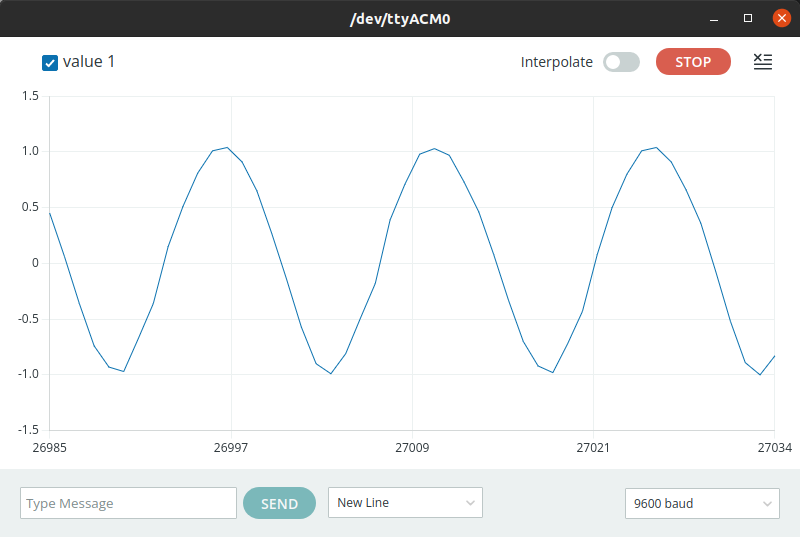
\includegraphics[width=0.85\textwidth]{images/microcontroller/sinewave-serial-plotter.png}
        \caption{Serial plotter.}
    \end{figure}
\end{frame}
\subsection{Control}
\begin{frame}
    \begin{listing}[H]
        \inputsource[firstline=13, lastline=20, highlightlines=18]{c}{arduino/sinewave.c}
        \caption{Project code: reduce frequency for better visibility.}
        \label{lst:arduino:tflite:sinewave:control:settings}
    \end{listing}
\end{frame}

\begin{frame}
    \begin{listing}[H]
        \inputsource[gobble=2, fontsize=\fontsize{10}{10}, firstline=107, lastline=131, highlightlines={107,111,126}]{c}{arduino/sinewave.c}
        \caption{Project code: infer sinus value from continuous input values.}
        \label{lst:arduino:tflite:sinewave:control:loop}
    \end{listing}
\end{frame}

\appendix

\begin{frame}[allowframebreaks]{Acronyms}
    \glsadd{ml}
    \printglossary[type=\acronymtype, nonumberlist]
\end{frame}

% \begin{frame}[label=references]{References}
%     \bibliography{references}
% \end{frame}

\end{document}